\chapter{Testing Results}
%TC:ignore

\label{appendix:test_results}
This appendix chapter shows the different sections of the application that has been tested and the test outcomes.


\section{Unit tests} \label{test:unit}
\subsection{Binarise image}
\begin{figure}[H]
  \centering
  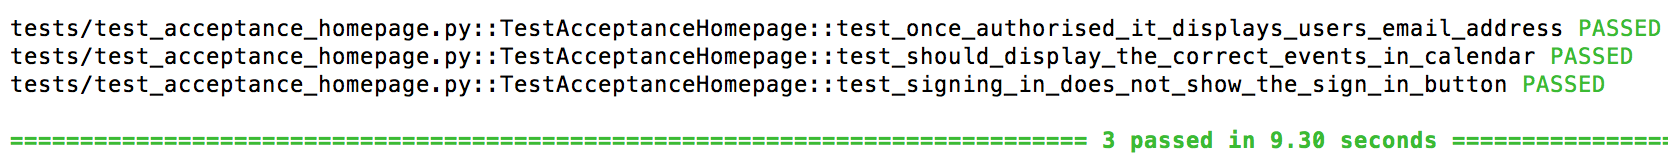
\includegraphics[width=\textwidth]{images/test_acceptance_homepage}
  \caption{Acceptance test being conducted for the homepage, to ensure that the homepage displays the correct content.}
  \label{fig:acceptance_homepage}
\end{figure}

\section{Acceptance tests} \label{tests:acceptance}
\label{appendix:acceptance}
The following section displays visual representation of the acceptance tests being executed, and their overall status.

\subsection{Add meta-data}

\begin{figure}[H]
  \centering
  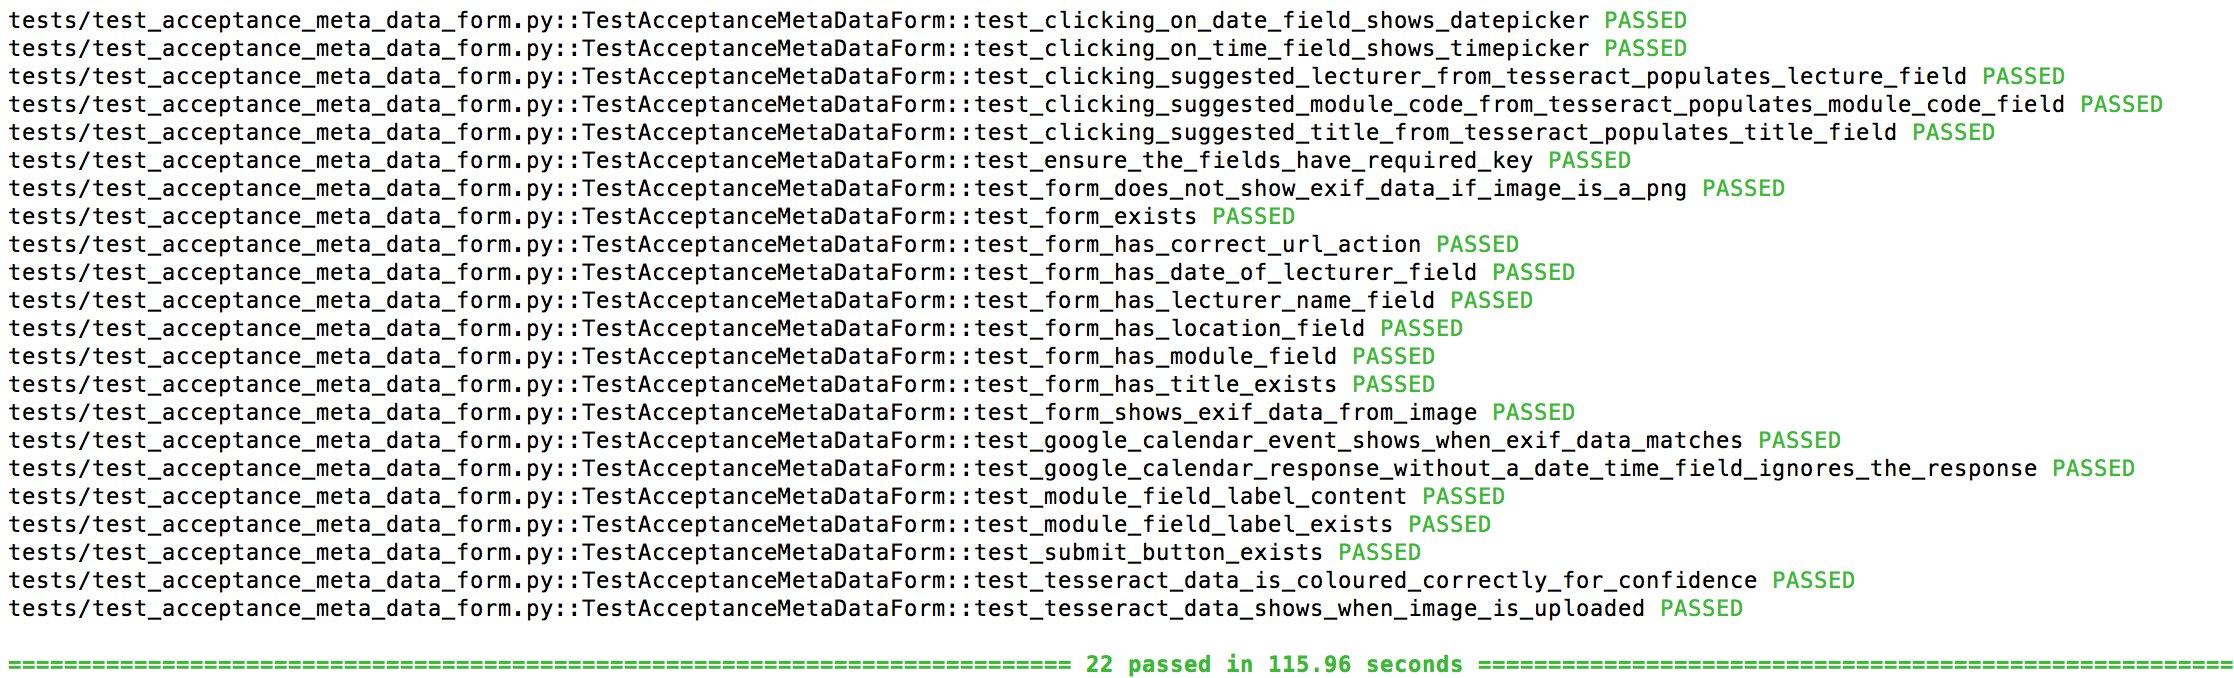
\includegraphics[width=\textwidth]{images/test_acceptance_meta_data_form}
  \caption{Acceptance test being performed to ensure that meta-data can be added to the correct note.}
  \label{fig:acceptance_add_meta_data}
\end{figure}

\subsection{Viewing all the notes}

\begin{figure}[H]
  \centering
  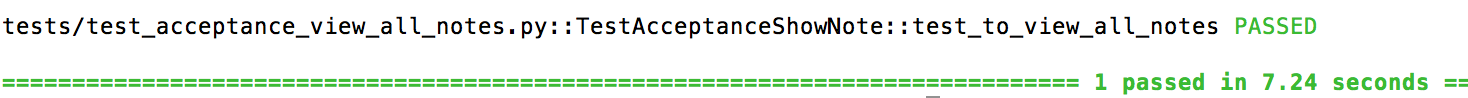
\includegraphics[width=\textwidth]{images/test_acceptance_view_notes}
  \caption{Acceptance test being conducted to ensure that all the notes can be viewed.}
  \label{fig:acceptance_view_note}
\end{figure}


\section{Integration tests}
\label{appendix:integration_tests}

\subsection{Add and edit meta data}
\begin{figure}[H]
  \centering
  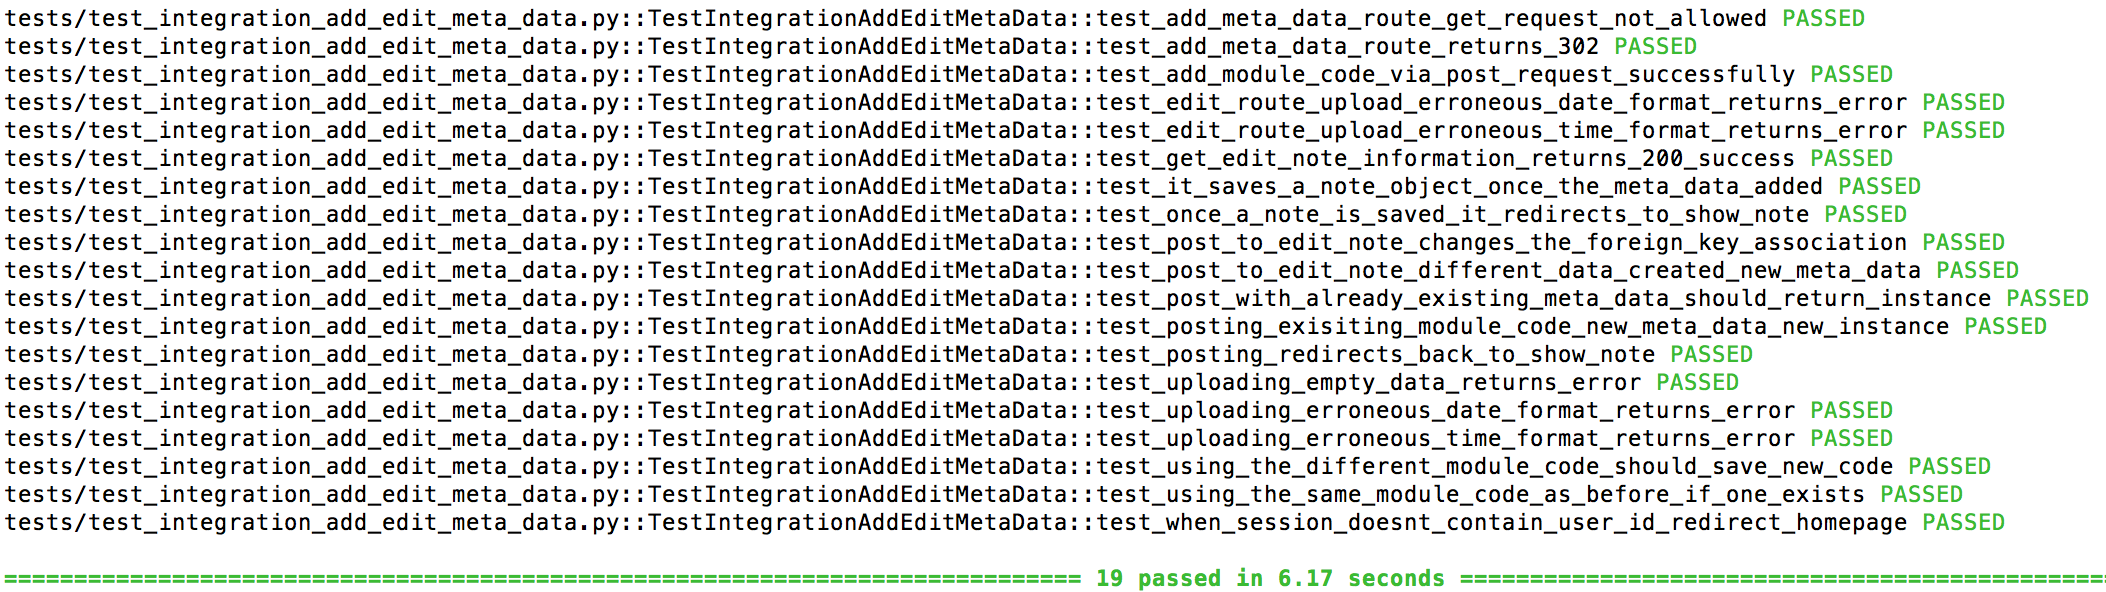
\includegraphics[width=\textwidth]{images/test_integration_add_edit_meta_data}
  \caption{Integration tests carried on the add and edit meta url to ensure the system worked well together.}
  \label{fig:integration_add_edit}
\end{figure}

\section{User study tests}
The following sections shows the results of the questionnaire  conducted for the user-study.

\noindent
\textbf{How easy was it to add a note?}
\begin{table}[h!]
\centering
 \begin{tabular}{|c c c c c c|}
 \hline
   Person & 1 & 2 & 3 & 4 & 5 \\ [0.5ex]
 \hline\hline
    1 & & & & x &  \\
    2 & & & & & x  \\
 \hline
  \end{tabular}
  \caption{On a scale of 1-5 (1 being very hard, 5 being very hard) how easy was it to add a note?}
\end{table}

\vspace{1em}
\noindent
\textbf{How easy was it to navigate around the application?}
\begin{table}[h!]
\centering
 \begin{tabular}{|c c c c c c|}
 \hline
   Person & 1 & 2 & 3 & 4 & 5 \\ [0.5ex]
 \hline\hline
    1 & & & & x &  \\
    2 & & & & & x  \\
 \hline
  \end{tabular}
  \caption{On a scale of 1-5 (1 being very hard, 5 being very hard) how easy was it to navigate around the application?}
\end{table}

\noindent
\textbf{How easy was it to add meta-data to your note?}
\begin{table}[h!]
\centering
 \begin{tabular}{|c c c c c c|}
 \hline
   Person & 1 & 2 & 3 & 4 & 5 \\ [0.5ex]
 \hline\hline
    1 & & & & x &  \\
    2 & & & & & x  \\
 \hline
  \end{tabular}
  \caption{On a scale of 1-5 (1 being very hard, 5 being very hard) How easy was it to add meta-data to your note?}
\end{table}

\noindent
\textbf{Did the application show all the meta-data you wanted?}
\begin{table}[h!]
\centering
 \begin{tabular}{|c c c|}
 \hline
   Person & yes & no \\ [0.5ex]
 \hline\hline
    1 & x &  \\
    2 & & x  \\
 \hline
  \end{tabular}
  \caption{Did the application show all the meta-data you wanted? - yes or no}
\end{table}

\noindent
\textbf{If not what do you think it needs to show?}

``Perhaps an indicator that no metadata could be found''

\noindent
\textbf{How easy was it to search for a note?}
\begin{table}[h!]
\centering
 \begin{tabular}{|c c c c c c|}
 \hline
   Person & 1 & 2 & 3 & 4 & 5 \\ [0.5ex]
 \hline\hline
    1 & & & & x &  \\
    2 & & & & & x  \\
 \hline
  \end{tabular}
  \caption{On a scale of 1-5 (1 being very hard, 5 being very hard) How easy was it to search for a note?}
\end{table}

\noindent
\textbf{Do you like the user interface?}
\begin{table}[h!]
\centering
 \begin{tabular}{|c c c|}
 \hline
   Person & yes & no \\ [0.5ex]
 \hline\hline
    1 & x &  \\
    2 & & x  \\
 \hline
  \end{tabular}
  \caption{Do you like the user interface? - yes or no}
\end{table}

\noindent
\textbf{Is there anything which is missing that should be included?}

``No''

\noindent
\textbf{General comments about the application}

``Great!''

\noindent
\textbf{Would you use this software to track your notes?}
\begin{table}[h!]
\centering
 \begin{tabular}{|c c c|}
 \hline
   Person & yes & no \\ [0.5ex]
 \hline\hline
    1 & x &  \\
    2 & & x  \\
 \hline
  \end{tabular}
  \caption{Would you use this software to track your notes? - yes or no}
\end{table}

\noindent
\textbf{Any reason for the above answer?}

``I type them up manually after lectures, which helps me memorise them''
%TC:endignore
